%*******************************************************************************
%****************************** Second Chapter *********************************
%*******************************************************************************

\chapter{Experimental Methods}

\section{Atomic Force Microscopy}
Atomic force microscopy  \nomenclature[z-AFM]{AFM}{Atomic Force Microscopy} is a non-destructive characterisation technique which employs a sharp tip mounted on a cantilever which is rastered across a sample surface. Tip-surface interactions result in changes cantilever position which are measured using the reflection of laser light reflecting off the cantilever and a four-quadrant photodetector as shown in Fig.\ref{2.1}.

\begin{figure}[h]
	\centering
	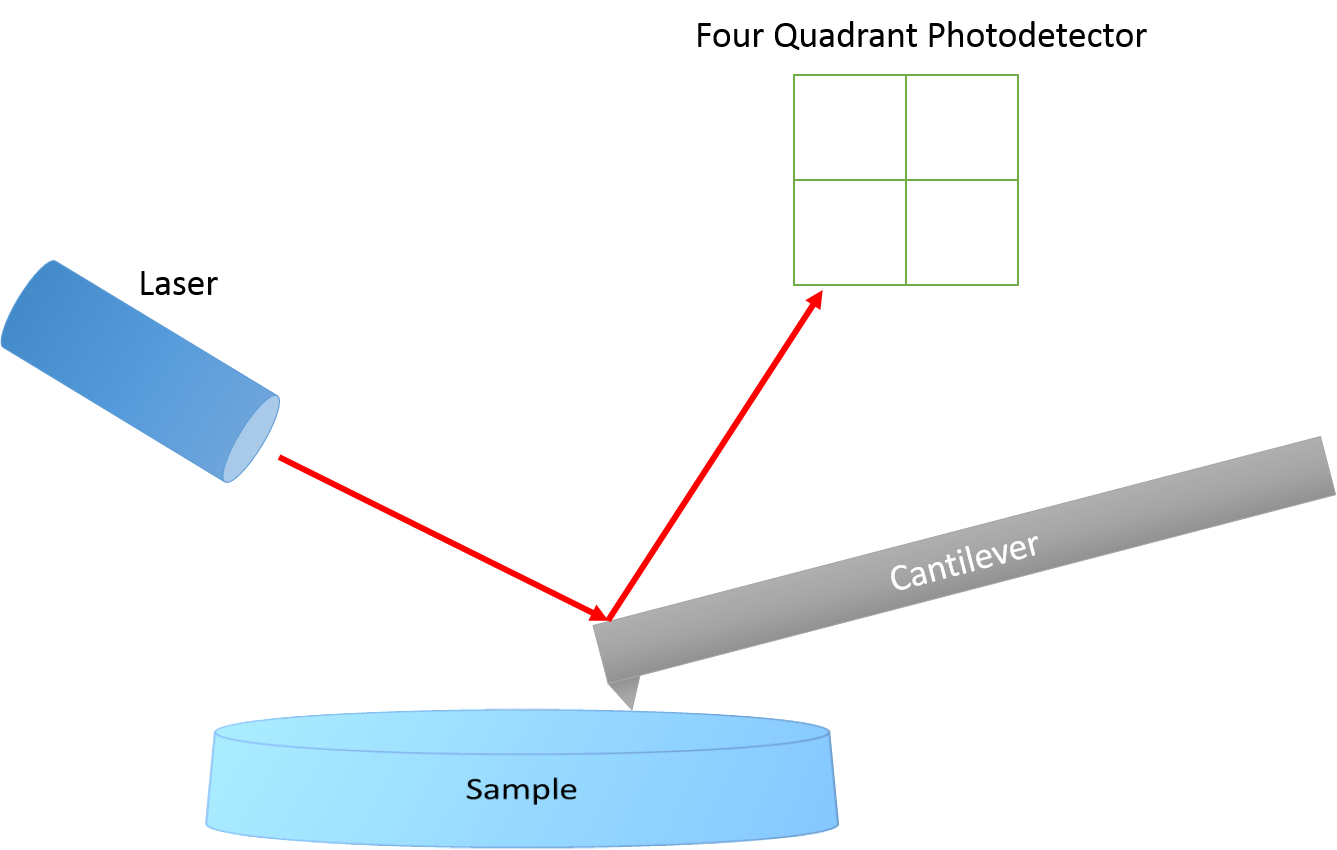
\includegraphics[width=0.7\textwidth]{Figs/Ch2/AFM.png}
	\caption {Schematic of an atomic force microscope.}
	\label{2.1}
\end{figure}
\FloatBarrier

The positioning and movement of the tip is achieved through the use of piezo-electric actuators. In contact mode, a feedback circuit is used to apply a voltage to the piezoelectric crystal in order to maintain a constant tip-sample separation should the tip encounter any features, thus avoiding damage to either the tip of sample. The voltage required to maintain this distance (also known as the setpoint) is registered at each pixel of the scan and is used in conjunction with calibration data to determine a vertical displacement value, thus generating a topographic image.\\
An alternative mode of operation known as tapping mode is often referred to contact mode. In this mode of operation the tip is made to oscillate close to its resonant frequency by the piezocrystal. Contact  between the tip and the sample is achieved at the lowest point of each oscillation, which damps the oscillation of the tip. The oscillation frequency is maintained by the piezoelectric crystal, thus allowing for the generation of a topographic map. Tapping mode is often preferred to contact mode due to the exclusion of lateral friction which can cause tip wear and sample damage.\\
The forces experienced by the tip vary depending on the tip-sample separation, as shown in Fig.\ref{2.2}. Van der Walls forces dominate at large separations attractive the tip to the surface. As the distance is reduced repulsive forces such as hard-sphere repulsion, electron-electron Coulomb interaction and the Pauli-exclusion interaction being to dominate. The sum of these forces result in cantilever deflection, changing the tip-sample interaction.

\begin{figure}[h]
	\centering
	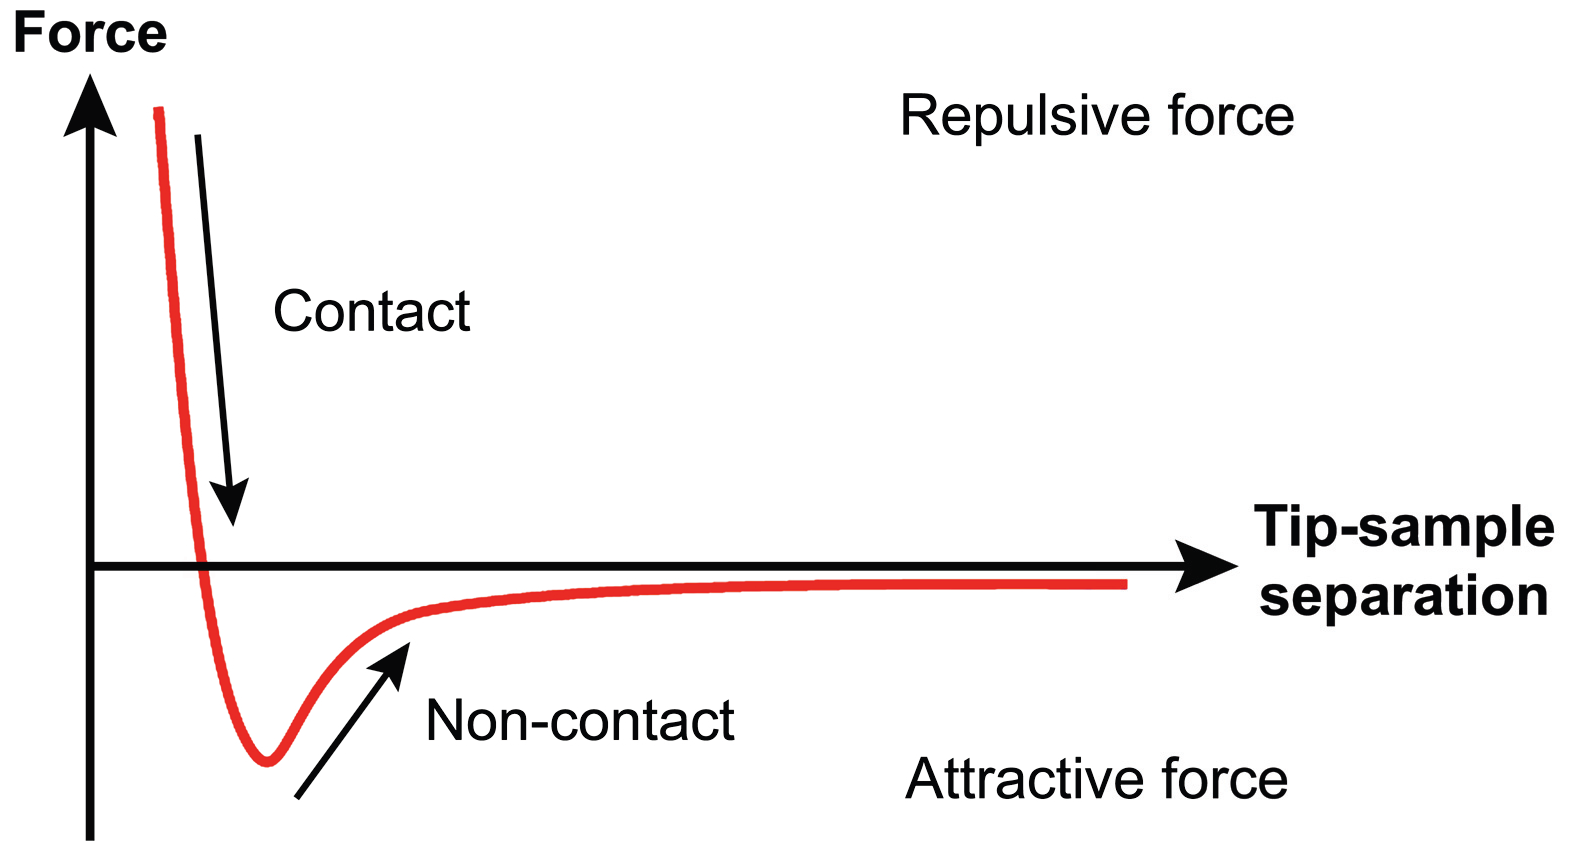
\includegraphics[width=0.7\textwidth]{Figs/Ch2/AFMint.png}
	\caption {The effect of separation on the tip-sample interaction force \cite{Zhu2010}.}
	\label{2.2}
\end{figure}
\FloatBarrier

AFM offers excellent vertical resolution limited only by the probes vertical movement and external noise. However, the lateral resolution of this microscopy technique is heavily dependent on the shape and size of the tip employed. This is perhaps best highlighted by Fig.\ref{2.3} which depicts a hemispherical tip scanning across a flat-topped island. The apex of the tip is in contact with the surface, but the side of the island also experiences some contact: in this case there is a distinction between the two cases shown in Fig.\ref{2.2}a) and b) as the error in the measured width of the island varies based on the relative size of the measured object to the tip.

\begin{figure}[h]
	\begin{subfigure}[t]{0.4\textwidth}
		\centering
		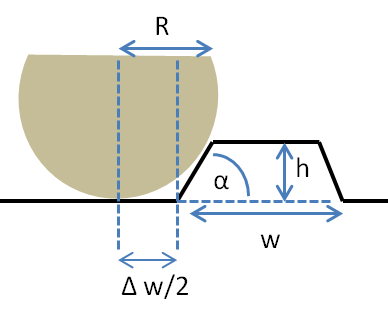
\includegraphics[width = 1\textwidth]{Figs/Ch2/afm1.png}
		\caption{}
	\end{subfigure}%
	\hspace*{1cm}
	~	
	\begin{subfigure}[t]{0.4\textwidth}
		\centering
		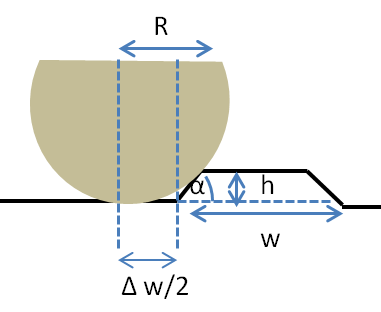
\includegraphics[width=1\textwidth]{Figs/Ch2/afm2.png}
		\caption{}
	\end{subfigure}
	\caption {Interaction of a hemisphere with a flat-topped island for the cases a) $h > R(1-cos(\alpha))$ and b) $h < R(1-cos(\alpha))$ adapted from \cite{Oliver2008}. }
	\label{2.3}
\end{figure}
\FloatBarrier 

Similarly, when measuring depth rather than height the ability of the tip to penetrate into the spaces being measured is also a crucial consideration, as shown in Fig.\ref{2.4}. Thus, increasing the gradient of the tip and minimizing the tip apex are descriable to reduce tip-related measurement artefacts when performing atomic force microscopy.

\begin{figure}[h]
	\centering
	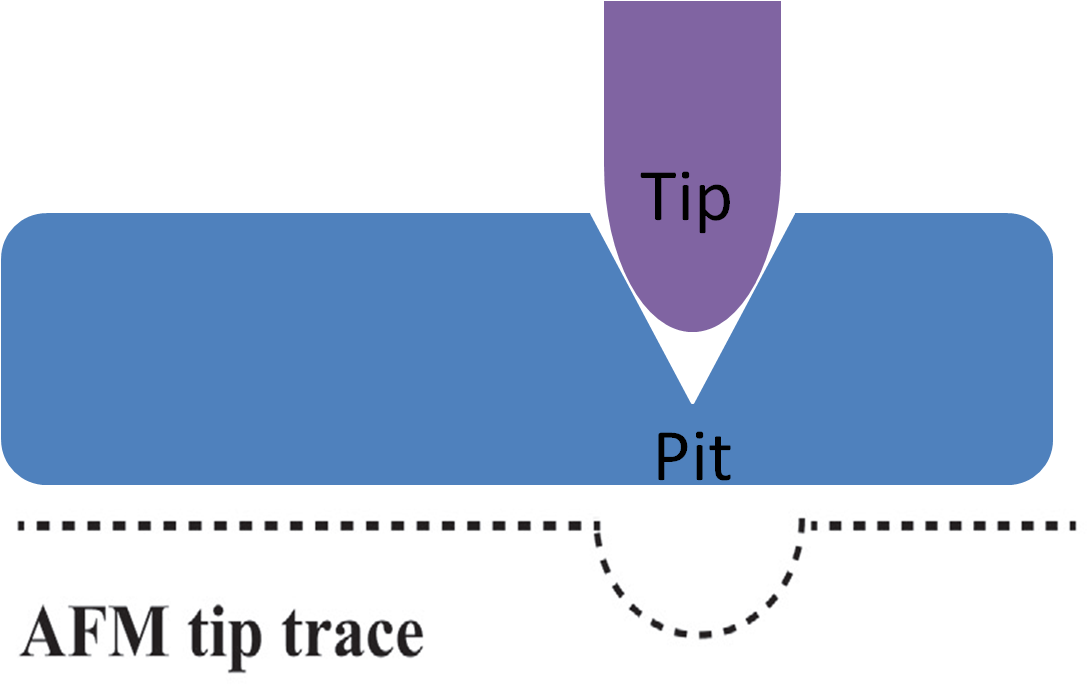
\includegraphics[width=0.4\textwidth]{Figs/Ch2/afm3.png}
	\caption {Measurement error in the depth of a pit caused by the finite width of the AFM tip.}
\end{figure}
\FloatBarrier

\subsubsection{Conductive Atomic Force Microcsopy}

Conductive atomic force microscopy \nomenclature[z-C-AFM]{C-AFM}{Conductive Atomic Force Microscopy} is a technique which combines AFM with local conductivity measurements. In order to perform C-AFM a conductive probe tip is brought close to contact with the sample and a bias is applied between the tip and the sample. The short tip-sample separation causes electron wavefunctions in the tip and sample to overlap, thus allowing a tunneling current to be generated through the application of a bias. C-AFM thus allows for the simultaneous measurement of tip-sample current flow and surface morphology, making it an extremely powerful tool to probe local sample conductivity. 


% Uncomment this line, when you have siunitx package loaded.
%The SI Units for dynamic viscosity is \si{\newton\second\per\metre\squared}.

\section{Hyperspectral Electroluminescence Mapping}
\section{Scanning Electron Microscopy and Cathodoluminescence}
\section{Photoluminescence}
\section{Dual Beam Scanning Electron microscopy with a Focussed Ion Beam}
\subsection{Fabrication}
\subsection{Tomography}
\section{Transmisson Electron Microscopy}
\subsection{Tomography}


